\chapter{Opis procesu}

\section{Opis ogólny}
Proces badany w pracy to linia montująca płyty drukowane do finalnych produktów.
Sam proces składa się z kilku etapów:
\begin{enumerate}
	\item Pobranie potrzebnych elementów elektronicznych z magazynu.
	\item Uzbrojenie automatu pick\&place w wymagane elementy.
	\item Pobranie gotowych płyt PCB (ang. Printed Circuit Board).
	\item Ręczne nałożenie pasty lutowniczej za pomocą sitodruku
	\item Uruchomienie procesu montażu elementów na maszynie pick\&place.
	\item (Opcjonalnie) Umieszczenie ręczne elementów
	\item Przeprowadzenie procesu lutowania w piecu.
	\item (Opcjonalnie) Lutowanie ręczne.
	\item Kontrola gotowej płyty PCB\@.
\end{enumerate}

Cechy procesu:
\begin{itemize}
	\item wszystkie procedury muszą być wykonane w ustalonej kolejności,
	\item proces wymaga operatorów,
	\item dla płyt dwustronnych należy powtórzyć sekwencję,
	\item automat pick\&place może obsługiwać tylko jedną płytę PCB,
	\item piec lutowniczy może lutować kilka płyt drukowanych (ilość jest zależna od rozmiaru płyt).
\end{itemize}

Cały przepływ pracy został przedstawiony na diagramie~\ref{DiagFlow}.
Czerwone krawędzie wyznaczają ścieżkę krytyczną procesu.
Węzły o krawędziach przerywanych są to operacje opcjonalne zależne od projektu płyty PCB\@.

\begin{figure}[H]
	\centering
	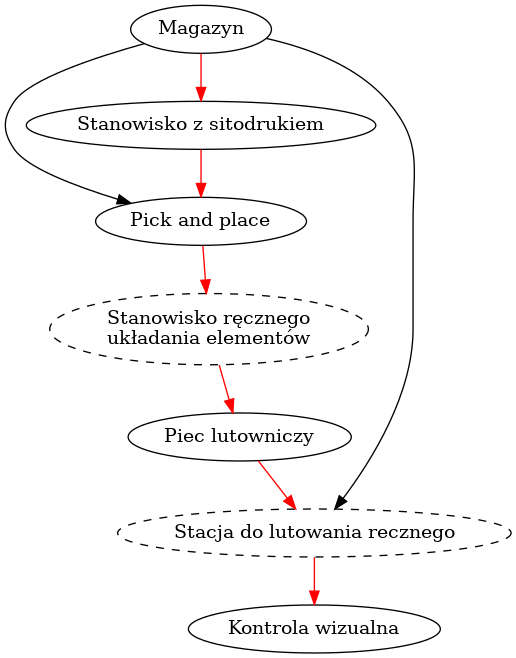
\includegraphics[scale=0.5]{./chapters/chapter2/diagram.png}
	\caption{Diagram przepływu pracy w procesie}
	\label{DiagFlow}
\end{figure}

\section{Opis stanowisk}

\subsection{Magazyn}
Magazyn jest miejscem od którego zaczyna się cały proces.
Przechowuje on wszystkie niezbędne elementy elektroniczne (rezystory, kondensatory, układy scalone itd.), gotowe płyty PCB oraz szablony sitodruku do poszczególnych projektów.
Aktualny stan magazynowy oraz fizyczna lokalizacja produktów znajduję się w systemie ERP\@.
Wszystkie potrzebne przedmioty są pobierane przez operatora.

\subsection{Stanowisko z sitodrukiem}
W kolejnym etapie produkcji gotowa płytka PCB trafia na urządzenie sitodruku.
Możemy wyszczególnić kilka typów takiej maszyny~\cite{sitodruk}:
\begin{itemize}
	\item sitodruk manualny --- najprostsza wersja urządzenia. Cały proces sprowadza się do ręcznego ustawienia szablonu na płytce oraz ręcznego nałożenia pasty przez operatora. Cechuję się gorszą jakością i powtarzalnością operacji w porównaniu do urządzeń poniżej.
	\item sitodruk półautomatyczny --- operator ustawia płytkę względem szablonu często przy pomocy systemu wizyjnego. Proces naniesienia pasty odbywa się automatycznie. Rozwiązanie to często się wykorzystuje przy prototypowaniu oraz produkcji małoseryjnej.
	\item sitodruk automatyczny --- rola operatora sprowadza się do podania płytki i odebrania po naniesieniu pasty (system offline) lub załadowania podajnika czystymi płytkami i później odebraniu gotowych (rozwiązanie in-line). Wszystkie czynności takie jak ustawienie szablonu i nałożenie pasty odbywają się automatycznie.
\end{itemize}

W naszym przypadku używany jest sitodruk manualny (Rysunek~\ref{sitodruk}). Operator przed nałożeniem pasty na płytę PCB musi przezbroić maszynę. Proceder polega na przyniesieniu szablonu z magazynu oraz ustawieniu go na maszynie. W dalszym kroku następuje manualne naniesienie pasty.

\begin{figure}[H]
	\centering
	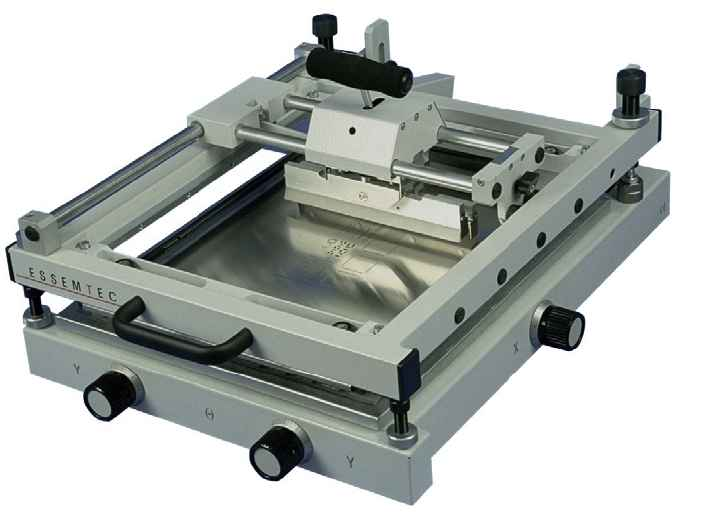
\includegraphics[scale=0.3]{./chapters/chapter2/sitodruk.jpg}
	\caption{Urządzenie sitodruku manualnego~\cite{sitodruk}}
	\label{sitodruk}
\end{figure}

\subsection{Automat pick\&place}
Automat pick and place to maszyna która umożliwia za pomocą systemu wizyjnego w precyzyjny sposób układać komponenty SMD na płytkach PCB~\cite{automatp&p}. W procesie badanym wykorzystywany jest automat (tu się doda model wykorzystywany w firmie, dorzucę jakieś zdjęcie oraz specyfikacje krótką)


\subsection{Stanowisk do ręcznego układania i lutowania elementów}
Stanowisko to posiada na wyposażeniu:
\begin{itemize}
	\item stację lutowniczą,
	\item stację hot-air,
	\item narzędzia drobne (szczypce, pęsety itd.),
	\item uchwyty montażowe,
	\item mikroskop.
\end{itemize}

\subsection{Piec lutowniczy}
(podobnie jak w pick\&place)
\subsection{Stanowisko z kontrolą wizualną}
